% A good introduction to latex can be found here:
%    http://www.cse.ohio-state.edu/~hank/latex/lshort141.pdf

\documentclass{article}

\usepackage{full page}  % make the margins somewhat smaller than the default

\usepackage{listings}  %  needed for source code listings
\usepackage{graphicx}
\lstset{language=Java}         

% set the document title, author, and date here.
%  once set, the \maketitle command (within the document)
%  will display them nicely
\title{Missionaries and Cannibals Solution}
\author{Michelle Shu}

\begin{document}
\maketitle

\section{Introduction}

In this assignment, I will address the problem of moving three missionaries and three cannibals across a river in a boat, under two constraints: (1) the boat can only carry one or two people at a time and (2) there cannot be more cannibals than missionaries on either side of the river at any time. All possible states of this system will be modeled as the tuple $(m, c, b)$, which indicates $m$ missionaries, $c$ cannibals and $b$ boats on the starting side of the river.

Not all states are legal, but if we do not consider the legality of states, we can derive an upper bound on the total number of possible states by considering all possible values of $(m, c, b)$. There can be $0$ to $3$ missionaries, $0$ to $3$ cannibals and either $0$ or $1$ boats on the starting side of the river. This gives us an upper bound of $4 * 4 * 2 = \bf{32}$ possible states.

\begin{figure}[!htb]
\centering
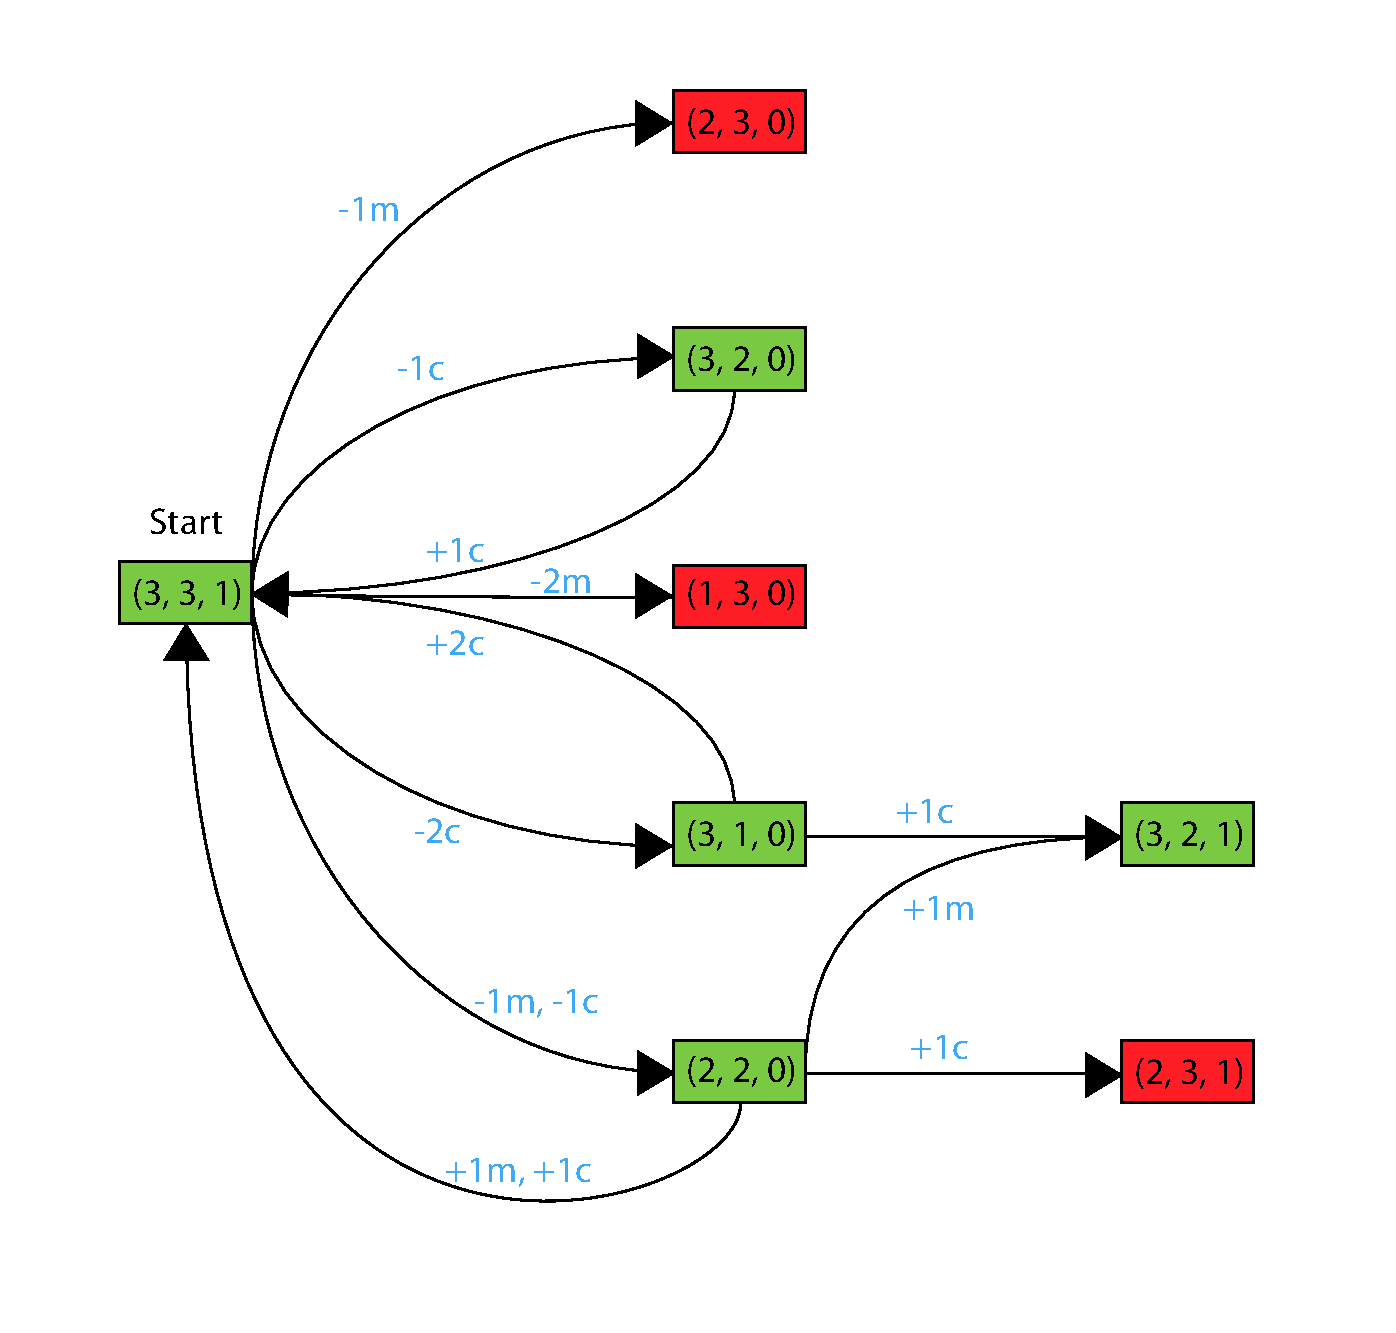
\includegraphics[scale=.45]{MCStates.pdf}
\caption{{\bf State Diagram.} Possible actions that can be taken up to two iterations out from start state. Green nodes indicate legal states, red nodes illegal ones. Blue action text represents change in number of people at start bank of river.}
\label{fig:MCStates}
\end{figure}

\section{Implementation of the model}

The model is implemented in 
\verb`CannibalProblem.java`.  Here's my code for \verb`getSuccessors`:

% Small trick -- dealing with tabs.  
%  When I copied from eclipse, there were large tabs in the pasted
%  text that made the following listing not fit on the page.  I did 
%  a search-and-replace, by copying a tab from this document into 
%  the "search" entry in the dialog box, and replacing with two spaces.

\begin{lstlisting}
// Get legal states reachable from current state using valid actions
public ArrayList<UUSearchNode> getSuccessors() {
  ArrayList<UUSearchNode> successors = new ArrayList<UUSearchNode>();
  
  int dmMax, dcMax; // maximum change in number of missionaries or cannibals
  int dir;  // direction of change (- toward goal, + toward start)
  int b;    // position of boat in next move
  
  if (this.state[2] == 0) { // boat on goal side of river
    dir = 1;
    b = 1;
    dmMax = Math.min(BOAT_SIZE, totalMissionaries - this.state[0]);
    dcMax = Math.min(BOAT_SIZE, totalCannibals - this.state[1]);
  } else { // boat on start side of river
    dir = -1;
    b = 0;
    dmMax = Math.min(BOAT_SIZE, this.state[0]);
    dcMax = Math.min(BOAT_SIZE, this.state[1]);
  }
  
  // Loop through all possible actions; add states to successors if legal
  for (int dm = 0; dm <= dmMax; dm++) {
    for (int dc = 0; dc <= Math.min(BOAT_SIZE - dm, dcMax); dc++) {
      if (dm + dc == 0) {
        continue;  // need at least one to row the boat
      }
      
      int mNew = this.state[0] + dir * dm;
      int nNew = this.state[1] + dir * dc;
      if (isSafeState(mNew, nNew)) {
        successors.add(new CannibalNode(mNew, nNew, b, this.depth + 1));
      }
    }
  }
  
  return successors;
}

\end{lstlisting}
 
 \vspace{10mm}
The function \verb`getSuccessors` first computes the upper bounds on the number of missionaries and cannibals that are available to move and can fit in the boat, as well as the direction of the next boat movement. It then uses this information to generate all possible successive actions. 

\verb`getSuccessors` must also check that taking each of these actions will result in a valid state (i.e. No missionaries will be eaten.) To validate states, I used the helper method \verb`isSafeState` that returns \verb`true` if there are no missionaries outnumbered by cannibals on either side of the river:

 \vspace{10mm}
 
\begin{lstlisting}
private boolean isSafeState(int m, int c) {
  // More cannibals than missionaries on start side?
  if ((c > m) && (m > 0)) {
    return false;
  }
  // More cannibals than missionaries on goal side?
  if ((totalCannibals - c > totalMissionaries - m) && 
      (totalMissionaries - m > 0)) {
    return false;
  }
  return true;
}

\end{lstlisting}

I wrote an additional method under the \verb`CannibalProblem` class called \verb`test` to check that `getSuccessors` displays the desired behavior when called on the $(3, 3, 1)$ problem in its initial state:

\begin{lstlisting}
public void test() {
  CannibalNode start = new CannibalNode(3, 3, 1, 0);
  ArrayList<UUSearchNode> successors = start.getSuccessors();
  for (UUSearchNode s : successors) {
    System.out.println(s);
  }
}
\end{lstlisting}

This particular test resulted in the output of successor nodes $(3, 2, 0)$, $(3, 1, 0)$ and $(2, 2, 0)$ at depth 1, which matches the expected result as determined in Figure 1. Running the same method starting with the nodes $(3, 1, 0)$ and $(2, 2, 0)$ also gave the expected results for those nodes.

\section{Breadth-first search}

My breadth-first search method makes use of two data structures: a queue (Java's LinkedList implementation) to keep track of the nodes to visit next and a hash table (HashMap) to keep track of which nodes have already been visited and where they were visited from (their predecessor nodes).

\begin{lstlisting}
public List<UUSearchNode> breadthFirstSearch() {
  resetStats();
  
  // Queue of nodes to visit next
  LinkedList<UUSearchNode> queue = new LinkedList<UUSearchNode>();
  // Track predecessors of visited nodes in shortest path
  HashMap<UUSearchNode, UUSearchNode> predecessorOf = 
      new HashMap<UUSearchNode, UUSearchNode>(); 
  
  queue.addLast(startNode);
  while (!queue.isEmpty()) {
    UUSearchNode n = queue.removeFirst();
    if (n.goalTest()) {  // goal found!
      return backchain(n, predecessorOf);
    }
    ArrayList<UUSearchNode> successors = n.getSuccessors();
    for (UUSearchNode s : successors) {
      if (! predecessorOf.containsKey(s)) {
        queue.addLast(s);
        predecessorOf.put(s, n);
        incrementNodeCount();
        updateMemory(queue.size() + predecessorOf.size());
      }
    }
  }
  return null;  // no goal found
}
\end{lstlisting}

The \verb`backchain` method then recovers the shortest path to the goal node from the predecessor hash table:

\begin{lstlisting}
private List<UUSearchNode> backchain(UUSearchNode node,
    HashMap<UUSearchNode, UUSearchNode> predecessorOf) {
  LinkedList<UUSearchNode> path = new LinkedList<UUSearchNode>();
  UUSearchNode current = node;
  while (visited.get(predecessorOf) != startNode) {
    path.addFirst(current);
    current = predecessorOf.get(current);
  }
  path.addFirst(current);
  path.addFirst(startNode);
  return path;
}
\end{lstlisting}

The following is the output of the above implementation of BFS on the (3, 3, 1) missionaries and cannibals problem. As a test of correctness, we can see that all the moves described in this path are indeed valid and that the first two steps match valid steps derived in Figure 1.

\vspace{5mm}

{\setlength{\parindent}{0cm}
bfs path length:  12 [(3, 3, 1), (3, 1, 0), (3, 2, 1), (3, 0, 0), (3, 1, 1), (1, 1, 0), (2, 2, 1), (0, 2, 0), (0, 3, 1), (0, 1, 0), (0, 2, 1), (0, 0, 0)]\\
Nodes explored during last search: 15\\
Maximum memory usage during last search: 17\\
--------}

\section{Memoizing depth-first search}

Recursive memoizing depth-first search also tracks the visited nodes in a HashSet, but does not need to track the predecessor nodes, as the path can be recovered while the recursion stack frames are unwound. Here is my code for the function \verb`depthFirstMemoizingSearch` and its recursive counterpart, \verb`dfsrm`:

\begin{lstlisting}
public LinkedList<UUSearchNode> depthFirstMemoizingSearch(int maxDepth) {
  resetStats(); 
  HashMap<UUSearchNode, Integer> visited = 
      new HashMap<UUSearchNode, Integer>();
  visited.put(startNode, 1);
  return dfsrm(startNode, visited, 0, maxDepth);
}

private LinkedList<UUSearchNode> dfsrm(UUSearchNode currentNode, 
      HashMap<UUSearchNode, Integer> visited, int depth, int maxDepth) {
  updateMemory(visited.size());
  incrementNodeCount();

  if (currentNode.goalTest()) { // Base case: We found the goal!
    LinkedList<UUSearchNode> path = new LinkedList<UUSearchNode>();
    path.add(currentNode);
    return path;
  }
  
  // Keep looking recursively through successors not already visited.
  if (depth < maxDepth) {
    ArrayList<UUSearchNode> successors = currentNode.getSuccessors();
    for (UUSearchNode s : successors) {
      if (! visited.containsKey(s)) {
        visited.put(s, 1);
        LinkedList<UUSearchNode> path = 
            dfsrm(s, visited, depth + 1, maxDepth);
        if (path != null) {
          path.addFirst(currentNode);
          return path;
        }
      }
    }
  }
  return null; // Goal not reachable from currentNode
}
\end{lstlisting}

The apparent base case for this recursive algorithm is the case in which \verb`dfsrm` is called on the goal node. In this case, it simply returns a path containing only the goal. Otherwise, if the current node is not the goal node, we must recurse. There are two recursive scenarios: either there exists a path from the current node to the goal node or there is no path from the current node to the goal. In this algorithm, I first check to see if the first scenario is true by recursively performing dfsrm on the current node's valid successors. If I encounter a path from any of the successors to the goal, I simply tack on the current node to the path and return it. If no path exists from any of the successors to the goal, there is also no path from the current node to the goal and I return $null$.

Due to the need to track all visited nodes, memoizing DFS does not confer a significant memory advantage over BFS. Both methods require $O(n)$ memory, where $n$ is the number of nodes in the graph. This is because in the worst case, the goal is the last node explored and at this time, the hash table storing the visited nodes contains all $n$ nodes.

This is the result of running my memoized DFS on our standard test case of (3, 3, 1). It finds the same path that BFS found, with similar memory usage:

\vspace{5mm}

{\setlength{\parindent}{0cm}
dfs memoizing path length: 12 [(3, 3, 1), (3, 1, 0), (3, 2, 1), (3, 0, 0), (3, 1, 1), (1, 1, 0), (2, 2, 1), (0, 2, 0), (0, 3, 1), (0, 1, 0), (0, 2, 1), (0, 0, 0)]\\
Nodes explored during last search: 13\\
Maximum memory usage during last search: 13\\
--------}

\section{Path-checking depth-first search}

The path-checking approach is similar to memoized DFS. The key difference is that with path-checking DFS, we only commit to memory a list of the current path being explored, rather than of all visited vertices. To accomplish this, I applied one minor change to my code for memoizing DFS: After I finish exploring from a node, I remove it from the hash set of nodes on the current path. Here is my recursive path-checking DFS function \verb`dfsrpc`:

\begin{lstlisting}
private LinkedList<UUSearchNode> dfsrpc(UUSearchNode currentNode, 
      HashSet<UUSearchNode> currentPath, int depth, int maxDepth) {
    updateMemory(currentPath.size());
    incrementNodeCount();
  
    if (currentNode.goalTest()) { // Base case: We found the goal!
      LinkedList<UUSearchNode> path = new LinkedList<UUSearchNode>();
      path.add(currentNode);
      return path;
    }
    
    // Keep looking recursively through successors not already visited.
    if (depth < maxDepth) {
      ArrayList<UUSearchNode> successors = currentNode.getSuccessors();
      for (UUSearchNode s : successors) {
        if (! currentPath.contains(s)) {
          currentPath.add(s);
          LinkedList<UUSearchNode> path = 
              dfsrpc(s, currentPath, depth + 1, maxDepth);
          if (path != null) {
            path.addFirst(currentNode);
            return path;
          }
          currentPath.remove(s);
        }
      }
    }
    return null; // Goal not reachable from currentNode
  }
\end{lstlisting}

Path-checking DFS uses considerably less memory, as at any time, it only needs to store at most the number of nodes in the longest path in the graph (BFS may need to store all nodes in the graph if all are visited before the search terminates). However, in some cases, path-checking DFS may take considerably more time to run, as it may explore from the same node more than once. Here is a simple example of such a scenario:

\begin{figure}[!htb]
\centering
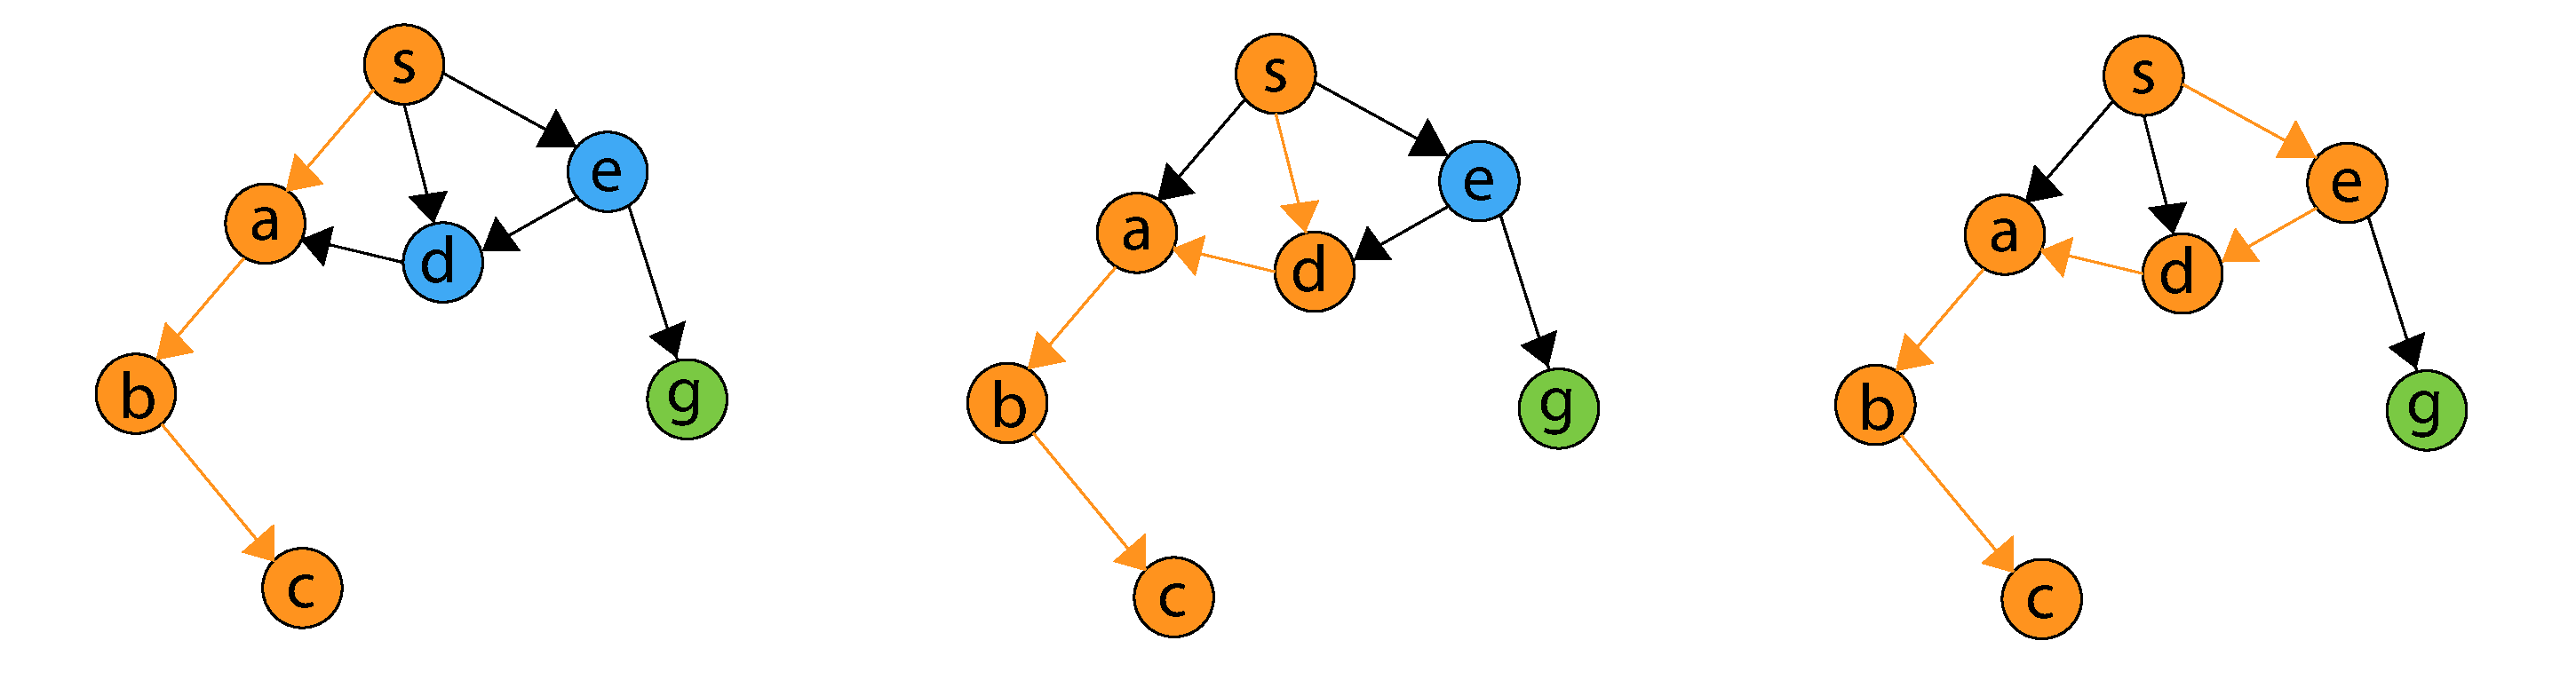
\includegraphics[scale=.35]{PCDFS.pdf}
\caption{{\bf Poor case for path-checking DFS.} In this case, nodes $a$, $b$, $c$ and $d$ are explored multiple times before the goal is found. BFS would only require looking at each node once, since it tracks all visited nodes.}
\label{fig:PCDFS}
\end{figure}

Running path-checking DFS on the (3, 3, 1) problem results in the following output:

\vspace{5mm}

{\setlength{\parindent}{0cm}
dfs path checking path length: 12 [(3, 3, 1), (3, 1, 0), (3, 2, 1), (3, 0, 0), (3, 1, 1), (1, 1, 0), (2, 2, 1), (0, 2, 0), (0, 3, 1), (0, 1, 0), (0, 2, 1), (0, 0, 0)]\\
Nodes explored during last search: 13\\
Maximum memory usage during last search: 12\\
--------}

We can better view the memory consumption advantage of path-checking DFS over BFS and memoizing DFS with the larger example problem of (10, 8, 1). (Note: Part of the reason BFS is shown to use so much memory is because it stores data in both the queue and the visited node hash table, but still it uses more than twice as much memory as the DFS path-checking method.)

\vspace{5mm}

{\setlength{\parindent}{0cm}
bfs path length:  34\\
Nodes explored during last search: 74\\
Maximum memory usage during last search: 77\\
--------\\
dfs memoizing path length: 36\\
Nodes explored during last search: 66\\
Maximum memory usage during last search: 66\\
--------\\
dfs path checking path length: 36\\
Nodes explored during last search: 72\\
Maximum memory usage during last search: 36\\
--------}\\

\section{Iterative deepening search}

Iterative deepening search is a method that guarantees that a shortest path is found by using multiple iterations of DFS, while imposing a depth limit that increases by one on each iteration. Only when the depth limit reaches the length of the shortest path to the goal will a path be returned, so the first path that is found is guaranteed to be a shortest path.

It is best to use path-checking DFS on each iteration of IDS to gain the extra advantage of less memory usage than BFS. At any given time, IDS with path-checking DFS will only need $O(d)$ space, where $d$ is the depth of the shortest path, whereas BFS requires $O(n)$ space, as shown previously. The time complexity of iterative deepening search is comparable to that of BFS and can be computed as follows: If $b$ is the branching factor of the tree, there are $b^d$ nodes at depth $d$ that are visited at most once (only during the last IDS iteration), $b^(d-1)$ nodes at depth $d - 1$ that are visited at most twice, and so on. So in total, we have at most:

\vspace{5mm}

$\sum\limits_{i=1}^d (d+1-i)*(b^i) = O(b^d)$ (due to the geometric series rule). 

\vspace{5mm}

This is comparable to BFS's time complexity of $O(n)$, since the number of nodes at depth $d$ is also $O(b^d)$. So in summary, iterative deepening search operates in roughly the same time as BFS, but consumes considerably less memory.

My code for iterative deepening search is the simple function \verb`IDSearch`, which makes use of the\\
 \verb`depthFirstPathCheckingSearch` function from the previous section:

\vspace{8mm}

\begin{lstlisting}
public LinkedList<UUSearchNode> IDSearch(int maxDepth) {
  resetStats();
  LinkedList<UUSearchNode> path = null;
  int depth = 0;
  while ((path == null) && (depth <= maxDepth)) {
    path = depthFirstPathCheckingSearch(depth);
    depth++;
  }
  return path;
}
\end{lstlisting}

As expected, it runs at about the same speed as BFS, but uses less memory. Here is a comparison of the results for the larger problem (10, 8, 1):

\vspace{5mm}

{\setlength{\parindent}{0cm}
bfs path length:  34\\
Nodes explored during last search: 74\\
Maximum memory usage during last search: 77\\
--------\\
Iterative deepening (path checking) path length: 34\\
Nodes explored during last search: 71\\
Maximum memory usage during last search: 34}\\


\section{Lossy missionaries and cannibals}

If a maximum of $E$ missionaries are willing to sacrifice themselves, the state space for this problem would expand. This new allowance would make it so that we could move into states that were previously illegal by sacrificing some missionaries during the search for the goal. We would also require another dimension in the state definition, indicating how many missionaries can still be sacrificed (initially $E$). Accordingly, the upper bound on the number of possible states would be $(m+1)*(c+1)*(b+1)*(E+1)$. The main change that would need to be made to the existing code is that the \verb`isSafeState` helper function for \verb`getSuccessor` would allow states in which some missionaries are eaten, as long as the total number of missionaries eaten is less than or equal to $E$. We would also need to keep track of the missionaries that have perished (4th dimension of state) when we take these actions.

\end{document}